% Degradation-aware amplitude-focused bandwidth extension with a Schrodinger bridge.
%
%   pdflatex architecture.tex   ->  architecture.pdf  (tightly cropped)
%   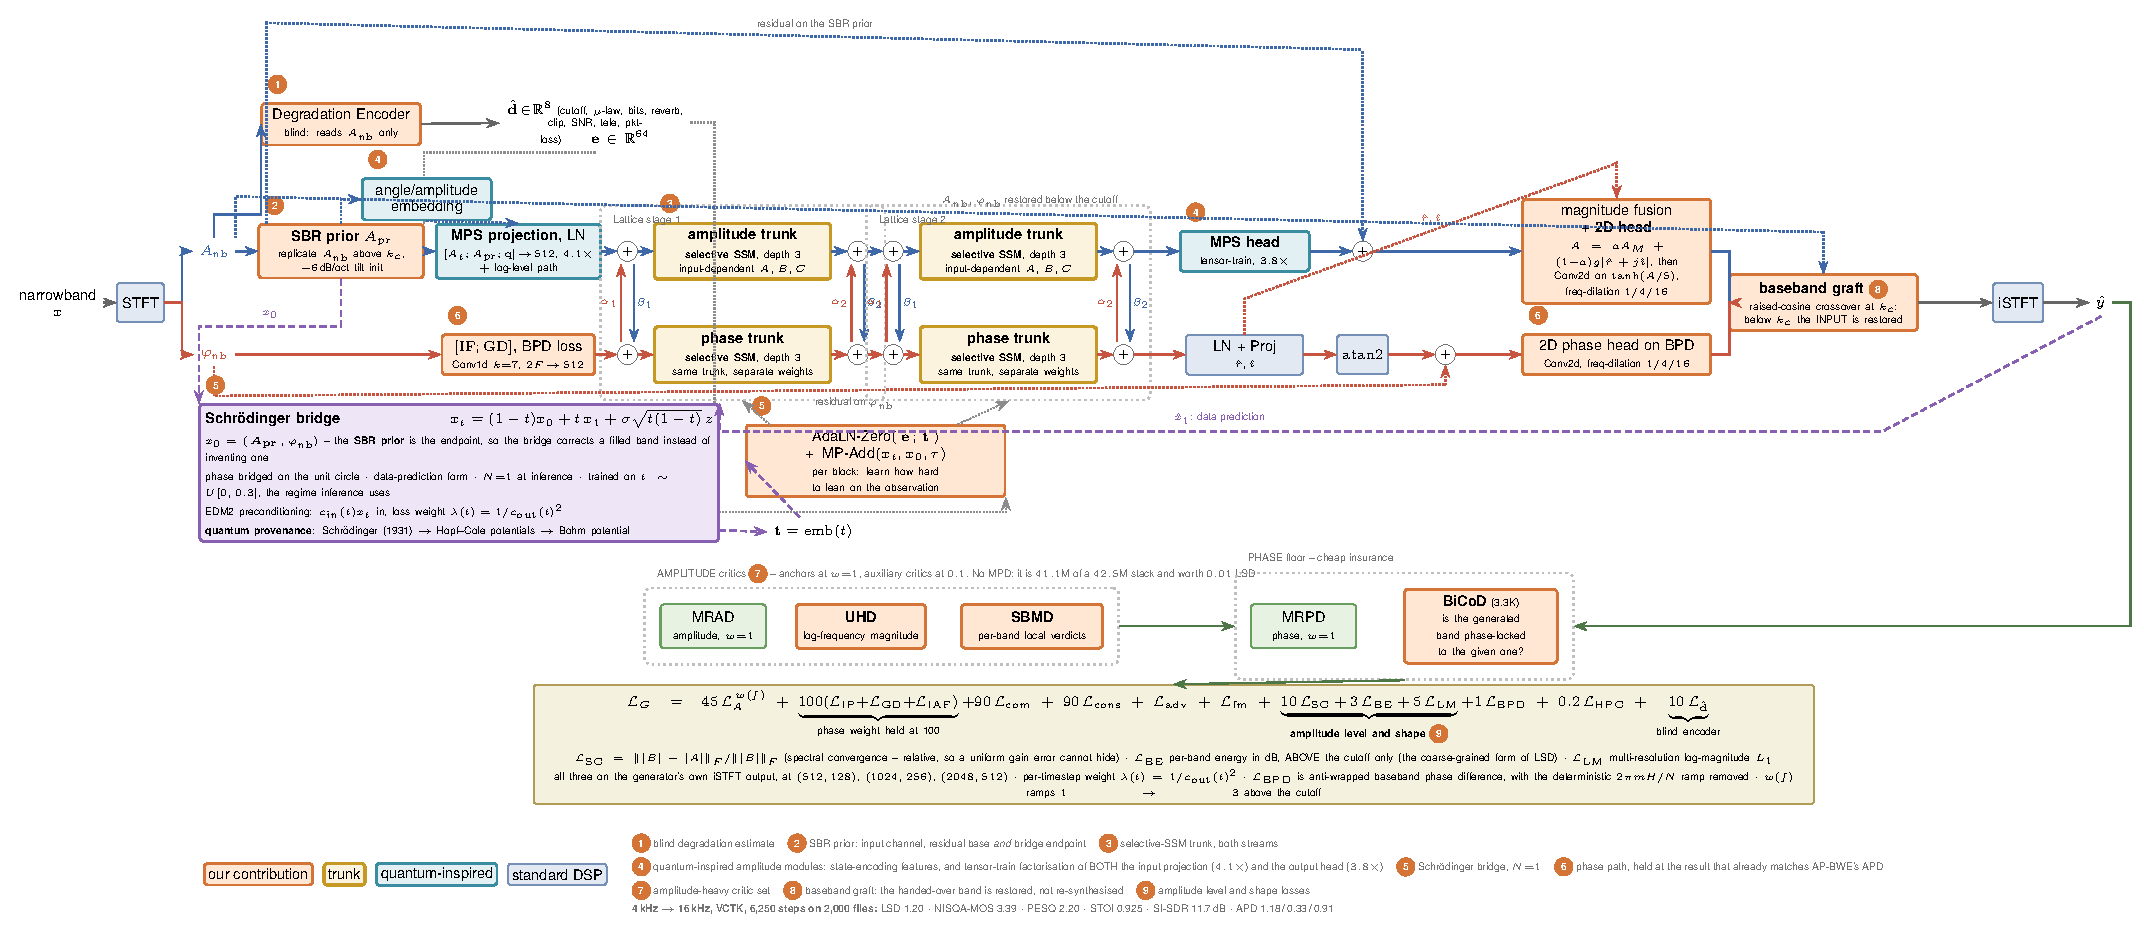
\includegraphics[width=\textwidth]{architecture.pdf}  inside a figure* environment
%
% READING THE FIGURE
%   solid orange  = our contribution
%   blue          = standard signal-processing blocks (STFT/iSTFT, projections)
%   This is the FINAL architecture: one model, no ablation axis. The trunk is a selective
%   state space in both streams.
\documentclass[border=6pt,tikz]{standalone}
\usepackage{amsmath,amssymb}
\usepackage{helvet}
\renewcommand{\familydefault}{\sfdefault}

\usepackage{tikz}
\usetikzlibrary{arrows.meta,positioning,fit,backgrounds,calc,shapes.geometric}

\definecolor{cCited}{RGB}{226,233,243}
\definecolor{cCitedL}{RGB}{116,144,182}
\definecolor{cOurs}{RGB}{255,231,211}
\definecolor{cOursL}{RGB}{212,116,54}
\definecolor{cMag}{RGB}{62,104,168}
\definecolor{cPha}{RGB}{198,84,64}
\definecolor{cAmp}{RGB}{252,243,222}
\definecolor{cAmpL}{RGB}{198,152,36}
\definecolor{cDisc}{RGB}{231,242,227}
\definecolor{cDiscL}{RGB}{104,158,96}
\definecolor{cLoss}{RGB}{245,241,223}
\definecolor{cLossL}{RGB}{176,156,86}
\definecolor{cBrg}{RGB}{238,229,246}
\definecolor{cBrgL}{RGB}{136,96,178}
\definecolor{cQ}{RGB}{226,240,244}
\definecolor{cQL}{RGB}{58,140,160}

\newcommand{\bdg}[1]{\tikz[baseline=(bc.base)]{\node[circle,fill=cOursL,text=white,
  font=\bfseries\tiny,inner sep=0.7pt,minimum size=3.1mm](bc){#1};}}

\begin{document}
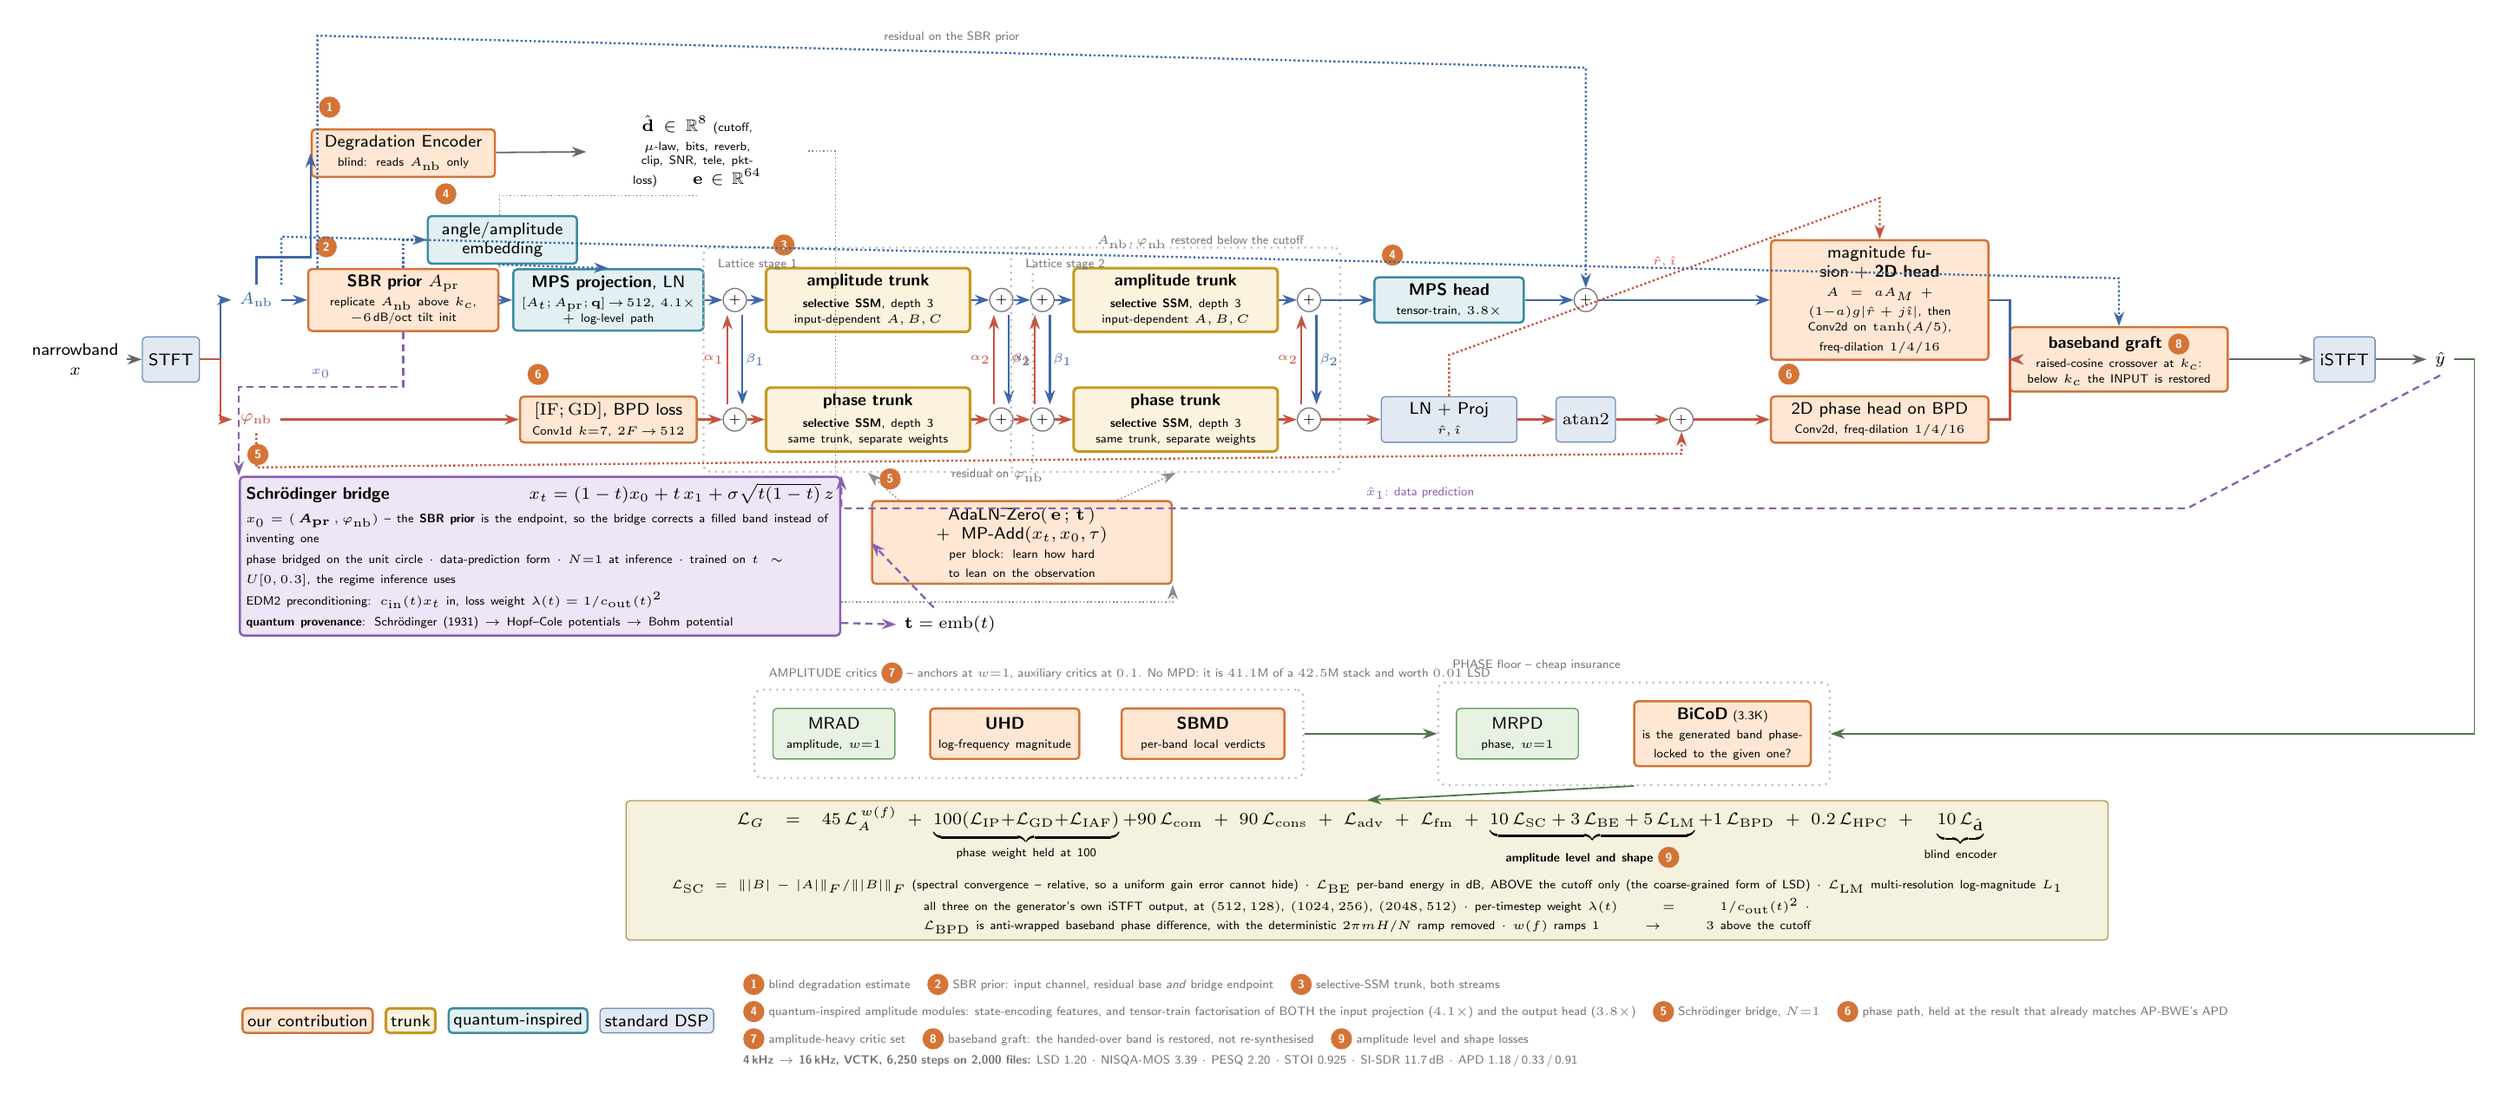
\begin{tikzpicture}[
  font=\scriptsize, >={Stealth[length=2.1mm,width=1.5mm]},
  bx/.style    ={rounded corners=1.6pt, line width=.5pt, align=center,
                 inner sep=2.6pt, minimum height=6.6mm},
  cit/.style   ={bx, draw=cCitedL, fill=cCited},
  ours/.style  ={bx, draw=cOursL,  fill=cOurs, line width=.9pt},
  todo/.style  ={bx, draw=cOursL,  fill=cOurs, line width=.9pt, densely dashed},
  amp/.style   ={bx, draw=cAmpL,   fill=cAmp,  line width=1.1pt},
  qq/.style    ={bx, draw=cQL,     fill=cQ,    line width=.9pt},
  disc/.style  ={bx, draw=cDiscL,  fill=cDisc, minimum height=7.4mm},
  loss/.style  ={bx, draw=cLossL,  fill=cLoss},
  brg/.style   ={bx, draw=cBrgL,   fill=cBrg,  line width=.9pt},
  op/.style    ={draw=black!55, fill=white, circle, inner sep=0.5pt,
                 line width=.45pt, minimum size=3.4mm, font=\tiny},
  mflow/.style ={->, draw=cMag, line width=.85pt},
  pflow/.style ={->, draw=cPha, line width=.85pt},
  flow/.style  ={->, draw=black!60, line width=.65pt},
  cond/.style  ={->, draw=black!45, line width=.55pt, densely dotted},
  cflow/.style ={->, draw=cBrgL, line width=.85pt, densely dashed},
  dflow/.style ={->, draw=cDiscL!75!black, line width=.65pt},
  grp/.style   ={draw=black!25, dotted, rounded corners=3pt, line width=.8pt},
  lbl/.style   ={font=\tiny, text=black!55},
]

\def\ym{0}        % amplitude row
\def\yp{-1.75}    % phase row

% ===================== analysis =====================================================
\node[align=center] (x) at (-1.5,-0.87) {narrowband\\$x$};
\node[cit] (stft) at (-0.1,-0.87) {STFT};
\draw[flow] (x) -- (stft);
\node[text=cMag] (anb) at (1.15,\ym) {$A_{\mathrm{nb}}$};
\node[text=cPha] (pnb) at (1.15,\yp) {$\varphi_{\mathrm{nb}}$};
\draw[mflow] (stft.east) -- ++(3mm,0) |- (anb.west);
\draw[pflow] (stft.east) -- ++(3mm,0) |- (pnb.west);

% ===================== (1) blind degradation + (2) SBR prior ========================
\node[ours, text width=25mm] (denc) at (3.3,2.15) {Degradation Encoder\\{\tiny blind: reads $A_{\mathrm{nb}}$ only}};
\node[above=0.3mm of denc.north west, anchor=south west] {\bdg{1}};
\node[align=center, text width=30mm] (desc) at (7.6,2.18)
  {$\hat{\mathbf d}\!\in\!\mathbb R^{8}$ {\tiny(cutoff, $\mu$-law, bits, reverb,}\\[-2pt]
   {\tiny clip, SNR, tele, pkt-loss)}\qquad $\mathbf e\!\in\!\mathbb R^{64}$};
\draw[mflow] (anb.north) -- ++(0,4mm) -| (denc.west);
\draw[flow] (denc) -- (desc);

\node[ours, text width=26mm] (prior) at (3.3,\ym) {\textbf{SBR prior} $A_{\mathrm{pr}}$\\{\tiny replicate $A_{\mathrm{nb}}$ above $k_c$,}\\[-1.5pt]{\tiny $-6$\,dB/oct tilt init}};
\node[above=0.3mm of prior.north west, anchor=south west] {\bdg{2}};
\draw[mflow] (anb) -- (prior);
\draw[cond] (desc.south) -| node[pos=.75,right,font=\tiny,text=black!55]{$k_c$} (prior.north east);

% ===================== stream front ends ============================================
\node[qq, text width=20mm] (qemb) at (4.75,0.88) {angle/amplitude\\embedding};
\node[above=0.3mm of qemb.north west, anchor=south west] {\bdg{4}};
\draw[mflow, densely dotted] (prior.north) |- (qemb.west);

\node[qq, text width=26mm] (prem) at (6.3,\ym) {\textbf{MPS projection}, LN\\{\tiny $[A_t;A_{\mathrm{pr}};\mathbf q]\!\to\!512$, $4.1\times$}\\[-1.5pt]{\tiny $+$ log-level path}};
\node[ours, text width=24mm] (prep) at (6.3,\yp) {$[\mathrm{IF};\mathrm{GD}]$, BPD loss\\{\tiny Conv1d $k{=}7$, $2F\!\to\!512$}};
\node[above=0.3mm of prep.north west, anchor=south west] {\bdg{6}};
\draw[mflow] (prior) -- (prem);
\draw[mflow, densely dotted] (qemb.south) -- (prem.north);
\draw[pflow] (pnb) -- (prep);

% ===================== Lattice stages ===============================================
\foreach \i/\xc in {1/10.1, 2/14.6}{
  \node[amp, text width=28mm] (cm\i) at (\xc,\ym)
    {\textbf{amplitude trunk}\\[1pt]{\tiny \textbf{selective SSM}, depth 3}\\[-1.5pt]
     {\tiny input-dependent $A,B,C$}};
  \node[amp, text width=28mm] (cp\i) at (\xc,\yp)
    {\textbf{phase trunk}\\[1pt]{\tiny \textbf{selective SSM}, depth 3}\\[-1.5pt]
     {\tiny same trunk, separate weights}};
  \node[op] (am\i) at (\xc-1.95,\ym) {$+$};
  \node[op] (ap\i) at (\xc-1.95,\yp) {$+$};
  \node[op] (bm\i) at (\xc+1.95,\ym) {$+$};
  \node[op] (bp\i) at (\xc+1.95,\yp) {$+$};
  \draw[mflow] (am\i) -- (cm\i);  \draw[mflow] (cm\i) -- (bm\i);
  \draw[pflow] (ap\i) -- (cp\i);  \draw[pflow] (cp\i) -- (bp\i);
  \draw[pflow] ($(ap\i)+(-1.1mm,2.2mm)$) -- node[pos=.5,left,font=\tiny,text=cPha,inner sep=1pt]{$\alpha_1$} ($(am\i)+(-1.1mm,-2.2mm)$);
  \draw[mflow] ($(am\i)+( 1.1mm,-2.2mm)$) -- node[pos=.5,right,font=\tiny,text=cMag,inner sep=1pt]{$\beta_1$} ($(ap\i)+( 1.1mm,2.2mm)$);
  \draw[pflow] ($(bp\i)+(-1.1mm,2.2mm)$) -- node[pos=.5,left,font=\tiny,text=cPha,inner sep=1pt]{$\alpha_2$} ($(bm\i)+(-1.1mm,-2.2mm)$);
  \draw[mflow] ($(bm\i)+( 1.1mm,-2.2mm)$) -- node[pos=.5,right,font=\tiny,text=cMag,inner sep=1pt]{$\beta_2$} ($(bp\i)+( 1.1mm,2.2mm)$);
  \node[grp, fit=(cm\i)(cp\i)(am\i)(bp\i), inner sep=2.8mm] (lat\i) {};
  \node[lbl, anchor=north west] at ($(lat\i.north west)+(1.0mm,-0.6mm)$) {Lattice stage \i};
}
\node[above=0.4mm of cm1.north west, anchor=south west] {\bdg{3}};
\draw[mflow] (prem) -- (am1);   \draw[pflow] (prep) -- (ap1);
\draw[mflow] (bm1) -- (am2);    \draw[pflow] (bp1) -- (ap2);

% ===================== conditioning =================================================
\node[ours, text width=42mm] (film) at (12.35,-3.55)
  {AdaLN-Zero$(\,\mathbf e\,;\,\mathbf t\,)$ \;+\; MP-Add$(x_t,x_0,\tau)$\\
   {\tiny per block: learn how hard to lean on the observation}};
\node[above=0.3mm of film.north west, anchor=south west] {\bdg{5}};
\draw[cond] (desc.east) -- ++(4mm,0) -- ++(0,-6.6) -| (film.south east);
\draw[cond] ($(film.north)+(-18mm,0)$) -- (lat1.south);
\draw[cond] ($(film.north)+( 14mm,0)$) -- (lat2.south);

% ===================== heads ========================================================
\node[qq, text width=20mm] (headm) at (18.6,\ym) {\textbf{MPS head}\\{\tiny tensor-train, $3.8\times$}};
\node[above=0.3mm of headm.north west, anchor=south west] {\bdg{4}};
\node[cit, text width=18mm] (headp) at (18.6,\yp) {LN + Proj\\{\tiny $\hat r,\hat\imath$}};
\draw[mflow] (bm2) -- (headm);  \draw[pflow] (bp2) -- (headp);
\node[op] (addm) at (20.6,\ym) {$+$};
\node[cit] (atan) at (20.6,\yp) {$\operatorname{atan2}$};
\draw[mflow] (headm) -- (addm);  \draw[pflow] (headp) -- (atan);
\node[op] (addp) at (22.0,\yp) {$+$};
\draw[pflow] (atan) -- (addp);
\draw[mflow, densely dotted] ($(prior.north west)+(1.5mm,0)$) -- ++(0,34mm)
  -- node[pos=.5,above,lbl]{residual on the SBR prior} ($(addm)+(0,34mm)$) -- (addm.north);
\draw[pflow, densely dotted] (pnb.south) -- ++(0,-5mm)
  -- node[pos=.52,below,lbl]{residual on $\varphi_{\mathrm{nb}}$} ($(addp)+(0,-5mm)$) -- (addp.south);

\node[ours, text width=30mm] (p2d) at (24.9,\yp) {2D phase head on BPD\\{\tiny Conv2d, freq-dilation $1/4/16$}};
\node[above=0.3mm of p2d.north west, anchor=south west] {\bdg{6}};
\draw[pflow] (addp) -- (p2d);
\node[ours, text width=30mm] (fuse) at (24.9,\ym) {magnitude fusion + \textbf{2D head}\\{\tiny $A=aA_M+(1{-}a)g|\hat r+j\hat\imath|$, then}\\[-1.5pt]{\tiny Conv2d on $\tanh(A/5)$, freq-dilation $1/4/16$}};
\draw[mflow] (addm) -- (fuse);
\draw[pflow, densely dotted] (headp.north) -- ++(0,6mm)
  -- node[pos=.5,above,font=\tiny,text=cPha]{$\hat r,\hat\imath$} ($(fuse.north)+(0,6mm)$) -- (fuse.north);

\node[ours, text width=30mm] (graft) at (28.4,-0.87)
  {\textbf{baseband graft} \bdg{8}\\{\tiny raised-cosine crossover at $k_c$:}\\[-1.5pt]
   {\tiny below $k_c$ the INPUT is restored}};
\draw[mflow] (fuse.east) -- ++(3mm,0) |- (graft.west);
\draw[pflow] (p2d.east)  -- ++(3mm,0) |- (graft.west);
\draw[mflow, densely dotted] (anb.north east) -- ++(0,7mm)
  -- node[pos=.5,above,lbl]{$A_{\mathrm{nb}},\varphi_{\mathrm{nb}}$ restored below the cutoff}
     ($(graft.north)+(0,7mm)$) -- (graft.north);
\node[cit] (istft) at (31.7,-0.87) {iSTFT};
\node (yh) at (33.1,-0.87) {$\hat y$};
\draw[flow] (graft) -- (istft);
\draw[flow] (istft) -- (yh);

% ===================== (5) Schrodinger bridge =======================================
\node[brg, text width=86mm, align=left] (bridge) at (5.3,-3.75)
  {\textbf{Schr\"odinger bridge}\hfill $x_t=(1-t)x_0+t\,x_1+\sigma\sqrt{t(1-t)}\,z$\\[2pt]
   {\tiny $x_0=(\,\boldsymbol{A_{\mathrm{pr}}}\,,\varphi_{\mathrm{nb}})$ -- the \textbf{SBR prior} is the endpoint, so the
    bridge corrects a filled band instead of inventing one}\\[1pt]
   {\tiny phase bridged on the unit circle $\cdot$ data-prediction form $\cdot$ $N{=}1$ at inference $\cdot$ trained on $t\sim U[0,0.3]$, the regime inference uses}\\[1pt]
   {\tiny EDM2 preconditioning: $c_{\mathrm{in}}(t)x_t$ in, loss weight $\lambda(t)=1/c_{\mathrm{out}}(t)^2$}\\[1pt]
   {\tiny \textbf{quantum provenance}: Schr\"odinger (1931) $\to$ Hopf--Cole potentials $\to$ Bohm potential}};
\node[above=0.3mm of bridge.north west, anchor=south west] {\bdg{5}};
\node[align=center] (temb) at (11.3,-4.75) {$\mathbf t=\mathrm{emb}(t)$};
\draw[cflow] ($(bridge.south east)+(0,2mm)$) -- (temb.west);
\draw[cflow] (temb) -- (film.west);
\draw[cflow] (prior.south) -- ++(0,-8mm) -| node[pos=.25,above,font=\tiny,text=cBrgL]{$x_0$} (bridge.north west);
\draw[cflow] (yh.south) -- (29.4,-3.05)
  -- node[pos=.57,above,font=\tiny,text=cBrgL]{$\hat x_1$: data prediction}
     (bridge.north east |- 29.4,-3.05) -- (bridge.north east);

% ===================== (7) critics ==================================================
\def\yd{-6.35}
\node[disc, text width=16mm] (mrad) at (9.6,\yd) {MRAD\\{\tiny amplitude, $w{=}1$}};
\node[ours, text width=20mm, minimum height=7.4mm] (uhd) at (12.1,\yd)
  {\textbf{UHD}\\{\tiny log-frequency magnitude}};
\node[ours, text width=22mm, minimum height=7.4mm] (sbmd) at (15.0,\yd)
  {\textbf{SBMD}\\{\tiny per-band local verdicts}};
\node[grp, fit=(mrad)(sbmd), inner sep=2.6mm] (agrp) {};
\node[lbl, anchor=west] at ($(agrp.north west)+(1mm,2.3mm)$)
  {AMPLITUDE critics \bdg{7} {\tiny-- anchors at $w{=}1$, auxiliary critics at $0.1$.
   No MPD: it is $41.1$M of a $42.5$M stack and worth $0.01$ LSD}};

\node[disc, text width=16mm] (mrpd) at (19.6,\yd) {MRPD\\{\tiny phase, $w{=}1$}};
\node[ours, text width=24mm, minimum height=7.4mm] (bicod) at (22.6,\yd)
  {\textbf{BiCoD}\;{\tiny(3.3K)}\\{\tiny is the generated band phase-locked to the given one?}};
\node[grp, fit=(mrpd)(bicod), inner sep=2.6mm] (pgrp) {};
\node[lbl, anchor=west] at ($(pgrp.north west)+(1mm,2.3mm)$) {PHASE floor -- cheap insurance};
\draw[dflow] (yh.east) -- ++(3mm,0) |- (pgrp.east);
\draw[dflow] (agrp.east) -- (pgrp.west);

% ===================== losses =======================================================
\node[loss, text width=215mm] (losses) at (17.4,-8.35)
  {$\mathcal L_G=
    45\,\mathcal L_{A}^{\,w(f)}
    +\underbrace{100\!\left(\mathcal L_{\mathrm{IP}}{+}\mathcal L_{\mathrm{GD}}{+}\mathcal L_{\mathrm{IAF}}\right)}_{\text{phase weight held at 100}}
    +90\,\mathcal L_{\mathrm{com}}+90\,\mathcal L_{\mathrm{cons}}
    +\mathcal L_{\mathrm{adv}}+\mathcal L_{\mathrm{fm}}
    +\underbrace{10\,\mathcal L_{\mathrm{SC}}+3\,\mathcal L_{\mathrm{BE}}+5\,\mathcal L_{\mathrm{LM}}}_{\textbf{amplitude level and shape}\;\bdg{9}}
    +1\,\mathcal L_{\mathrm{BPD}}+0.2\,\mathcal L_{\mathrm{HPC}}
    +\underbrace{10\,\mathcal L_{\hat{\mathbf d}}}_{\text{blind encoder}}$\\[3pt]
   {\tiny $\mathcal L_{\mathrm{SC}}=\lVert|B|-|A|\rVert_F/\lVert|B|\rVert_F$ (spectral convergence -- relative, so a
    uniform gain error cannot hide) $\cdot$
    $\mathcal L_{\mathrm{BE}}$ per-band energy in dB, ABOVE the cutoff only (the coarse-grained form of LSD) $\cdot$
    $\mathcal L_{\mathrm{LM}}$ multi-resolution log-magnitude $L_1$}\\[1pt]
   {\tiny all three on the generator's own iSTFT output, at $(512,128)$, $(1024,256)$,
    $(2048,512)$ $\cdot$ per-timestep weight $\lambda(t)=1/c_{\mathrm{out}}(t)^2$ $\cdot$
    $\mathcal L_{\mathrm{BPD}}$ is anti-wrapped baseband phase difference, with the
    deterministic $2\pi mH/N$ ramp removed $\cdot$ $w(f)$ ramps $1\to3$ above the cutoff}};
\draw[dflow] (pgrp.south) -- (losses.north);

% ===================== legend =======================================================
\node[ours, minimum height=3.6mm, inner sep=2pt] (lg1) at (1.9,-10.55) {our contribution};
\node[amp,  minimum height=3.6mm, inner sep=2pt, right=1.6mm of lg1] (lg2) {trunk};
\node[qq,   minimum height=3.6mm, inner sep=2pt, right=1.6mm of lg2] (lg3) {quantum-inspired};
\node[cit,  minimum height=3.6mm, inner sep=2pt, right=1.6mm of lg3] (lg4) {standard DSP};
\node[lbl, right=3mm of lg4, align=left]
  {\bdg{1} blind degradation estimate \quad \bdg{2} SBR prior: input channel, residual
   base \emph{and} bridge endpoint \quad \bdg{3} selective-SSM trunk, both streams\\[1.5pt]
   \bdg{4} quantum-inspired amplitude modules: state-encoding features, and tensor-train
   factorisation of BOTH the input projection ($4.1\times$) and the output head
   ($3.8\times$) \quad \bdg{5} Schr\"odinger bridge, $N{=}1$ \quad \bdg{6} phase path, held at
   the result that already matches AP-BWE's APD\\[1.5pt]
   \bdg{7} amplitude-heavy critic set \quad \bdg{8} baseband graft: the handed-over band
   is restored, not re-synthesised \quad \bdg{9} amplitude level and shape losses\\[1.5pt]
   \textbf{4\,kHz $\to$ 16\,kHz, VCTK, 6{,}250 steps on 2{,}000 files:} LSD 1.20 $\cdot$ NISQA-MOS 3.39 $\cdot$ PESQ 2.20 $\cdot$ STOI 0.925 $\cdot$ SI-SDR 11.7\,dB $\cdot$ APD 1.18\,/\,0.33\,/\,0.91};

\end{tikzpicture}
\end{document}
